\documentclass[11pt,a4paper]{article}
\usepackage[margin=1in]{geometry}
\usepackage{hyperref}
\usepackage{enumitem}
\usepackage{graphicx}
\usepackage{xcolor}
\usepackage{booktabs}
\usepackage{tikz}
\usetikzlibrary{arrows.meta,positioning,fit,backgrounds}

% -----------------------------------------------------
% bvraghav-tiet-ucs503p-article.sty
% -----------------------------------------------------

% Variable: Lab Instructor
\makeatletter \newcommand{\BvrSetLabInstructor}[1]{%
  \gdef\Bvr@LabInstructor{#1}}
% default
\newcommand{\Bvr@LabInstructor}{Dr. Raghav %
  B. Venkataramaiyer}
% public accessor
\newcommand{\BvrLabInstructorValue}{\Bvr@LabInstructor}
\makeatother

% Add subtitle
\usepackage{titling}
% -- Set title bold
\pretitle{\begin{center}\bfseries\fontsize{18bp}{18bp}\selectfont}
\makeatletter
\newcommand{\BvrSubtitle}[1]{%
  \posttitle{%
    \par\end{center}
    \begin{center}\large#1\end{center}
    \vskip 0.5em}%
}
\makeatother

% Hints in the section title(s)
\newcommand{\BvrHint}[1]{%
  {\normalfont\normalsize\itshape\hfill #1}}

% -----------------------------------------------------
% Measured baselines, 2026-05-15 to 2026-08-14, at the
% Model Town, Patiala station. Produced by
% scripts/bootstrap.py and scripts/diagnose.py.
\newcommand{\ObsMean}{24.6}
\newcommand{\PersMAE}{6.5}
\newcommand{\ClimMAE}{9.8}
\newcommand{\CamsMAE}{52.3}
\newcommand{\CamsFitMAE}{8.5}
\newcommand{\CamsRatio}{3.13}
\newcommand{\CamsCorr}{0.38}
\newcommand{\NDays}{91}

% -----------------------------------------------------

\title{Pawan: Locally Calibrated Next-Day Air Quality
  Forecasting for Patiala}

\BvrSetLabInstructor{Dr. Raghav B. Venkataramaiyer}

\BvrSubtitle{%
  Statistical correction of a global forecast using
  station observations and upwind fire activity
  \\[0.4em]
  Project Proposal for UCS503P  \\
  Submitted to: \BvrLabInstructorValue \\ \bfseries
  Thapar Institute of Engineering and Technology%
}

\author{
  Gurkirpa Singh, CSED%
  \thanks{Roll No: \texttt{1024170378}, %
    Email: \texttt{gsarao\_be24\@thapar.edu}}
  \and
  Ketubh, CSED%
  \thanks{Roll No: \texttt{1024170399}, %
    Email: \texttt{kketubh1\_be24\@thapar.edu}}
  \and
  Aayush, CSED%
  \thanks{Roll No: \texttt{1024170379}, %
    Email: \texttt{akandhol\_be24\@thapar.edu}}
}

\date{\today}

\begin{document}
\maketitle

\section{Higher-order goal%
  \BvrHint{\ldots secondary framing}}
Every year between October and December, air quality
across Punjab deteriorates sharply as paddy residue is
cleared by burning. The wider problem, exposure to
seasonal air pollution, is a matter of agricultural
policy and public health, and no software project is
going to solve it.

What software can do is smaller and more definite. If
people knew a day in advance that tomorrow would be
bad, some of what they do outdoors could be moved.
Schools, sports coaching, construction supervision and
morning exercise all involve decisions taken the
previous evening. Those decisions are only as good as
the forecast behind them.

The engineering objective, therefore, is to make
next-day air quality information locally accurate for
one city, to deliver it reliably without human
intervention, and to be honest about how accurate it
actually is.

\section{Time-to-value %
\BvrHint{\ldots primary heuristic}}
\begin{itemize}[leftmargin=0.7cm]
  \item The baseline against which we will be judged can
    be computed from public archives in week one. It
    needs no users, no interviews and no field study. We
    therefore know the ``before'' number before any
    development starts.
  \item Data collection is automated in week two. After
    that the training set grows on its own, and every
    later iteration begins with more data than the one
    before it, whether or not anyone touched the
    repository that week.
  \item Each iteration adds one feature or one modelling
    change, and reports the change in error on a fixed
    held-out period. Progress in a given week is
    therefore a number, not a claim.
  \item The first iteration succeeds if it beats a naive
    persistence forecast. The second succeeds if it
    beats the global model we are correcting. Neither
    milestone depends on anyone adopting the system.
\end{itemize}

\section{Problem Statement}
Freely available air quality forecasts for Patiala come
from global atmospheric models. The one that underlies
most of them, the Copernicus Atmosphere Monitoring
Service (CAMS) global model, runs at a resolution of
about $0.4^\circ$, which is roughly $45$~km per grid
cell.

Patiala fits inside a single cell, with room to spare.
So does the surrounding farmland, and a stretch of
highway. The model treats all of it as one body of air
and reports one number. When we queried the source at
the station coordinates, the nearest grid point returned
was $30.30^\circ$N, $76.40^\circ$E, and the value at
that point is an average over an area far larger than
the city.

Four consequences follow.

\begin{itemize}[leftmargin=0.7cm]
  \item \textbf{The city is invisible to the model.}
    Local emission sources, land use and terrain lie
    below the grid scale and cannot be represented at
    all.
  \item \textbf{The resulting error is systematic.}
    Because it arises from fixed local factors rather
    than from chance, it repeats. Anything that repeats
    can be learned and subtracted.
  \item \textbf{The error is worst when it matters
    most.} During the burning season, concentrations are
    driven by transient plumes carried from upwind
    fields. A coarse model resolves these poorly, so
    forecast quality degrades in precisely the weeks
    when a warning would be useful.
  \item \textbf{Nobody is checking.} No forecast
    published for Patiala is routinely scored against
    the city's own monitoring station, so a reader has
    no basis for deciding how much to trust it.
\end{itemize}

\subsection{What we measured}
Before proposing anything we scored the global forecast against
the station's own record over \NDays{} days, from 15 May to 14
August 2026. The result is worse than we expected.

\begin{itemize}[leftmargin=0.7cm]
  \item The observed daily mean was \ObsMean~$\mu$g/m$^3$. The
    CAMS forecast for the same days averaged
    $\CamsRatio\times$ higher, a signed bias of
    $+\CamsMAE~\mu$g/m$^3$.
  \item Correlation between forecast and observation was
    $r=\CamsCorr$, so roughly $15\%$ of the variance in observed
    concentration is explained by the global forecast.
  \item Rescaling the forecast optimally, by fitting a straight
    line from forecast to observation on the same data, reduces
    its error to \CamsFitMAE~$\mu$g/m$^3$. That is still worse
    than assuming tomorrow resembles today, which achieves
    \PersMAE.
\end{itemize}

The conclusion shapes the whole project. The global forecast is
not merely miscalibrated at this station, it is weakly
informative. A correction that uses the forecast alone cannot
succeed. What is needed is a local model in which recent
observations carry the forecast, and the global model,
meteorology and upwind fire activity contribute additional
information at the margin.

\textbf{Why this problem, in this place, now.} Patiala
has a continuous ambient air quality monitoring station
at Model Town, operated by the Punjab Pollution Control
Board, whose hourly readings are published nationally.
Ground truth is already available and costs nothing.
Equally relevant, the project window runs from August to
December, which contains the burning season in full. The
system will be built before the event, deployed during
it, and evaluated against it. That alignment is
unusually favourable and is a large part of why we chose
this problem.

\section{Proposed Solution %
\BvrHint{\ldots Software Proposition}}

\subsection{Overview}
We propose a \textbf{web-based} service that forecasts
tomorrow's concentration at one station, using every signal
available on the previous evening. Recent observations at the
station form the backbone, since they are the strongest single
predictor. The global forecast, the local meteorological
forecast and upwind fire activity are additional inputs, each
retained only if it demonstrably reduces error.

We do not attempt to replace the global model. Replacing it
would be a research project, and a hopeless one at this scale.
Nor do we treat it as authoritative, because our own
measurements show it is not. We treat it as one input among
several, and we say by how much it helps.

\begin{itemize}[leftmargin=0.7cm]
  \item \textbf{Automated ingestion.} A scheduled job
    collects the previous day's observed concentrations,
    the forecast issued for the coming day, the local
    meteorological forecast, and satellite fire
    detections over the upwind region.
  \item \textbf{Feature assembly.} A reproducible
    transformation from raw records to a modelling
    table, with the forecast issue time carried on every
    row.
  \item \textbf{Correction model.} A supervised
    regression that predicts tomorrow's mean
    concentration from the global forecast plus local
    context.
  \item \textbf{Evaluation harness.} A rolling-origin
    backtest that scores the model and every baseline
    over the same periods, so comparisons are like for
    like.
  \item \textbf{Public dashboard.} One page: tomorrow's
    corrected forecast beside the uncorrected one,
    recent observations, current accuracy, and the
    timestamp of the last successful pipeline run.
  \item \textbf{Advisory layer.} A rule converting the
    predicted concentration into an air quality band and
    a short scheduling recommendation.
\end{itemize}

\subsection{Core workflow}
\begin{enumerate}[leftmargin=0.7cm]
  \item The scheduled job runs each morning and appends
    one record: yesterday's observation, the forecast
    issued for the coming day, the meteorological
    forecast, and the upwind fire count.
  \item The feature builder assembles a modelling table
    from the accumulated records, admitting only
    quantities that existed at forecast issue time.
  \item The model is fitted on the historical portion of
    that table and emits a corrected value for the next
    day.
  \item The backtest scores model and baselines on a
    held-out period and writes the metrics to a file.
  \item The dashboard is rebuilt from the prediction and
    metric files, so what is published always matches
    the last successful run.
\end{enumerate}

\subsection{Operating constraints we have imposed}
\begin{itemize}[leftmargin=0.7cm]
  \item Every data source must be free and publicly
    reachable, with no institutional permission
    required. We verified this experimentally before
    writing this proposal rather than assuming it.
  \item The system must run unattended. Any step that
    needs a person on a given morning is a defect, not a
    workflow.
  \item No new algorithm is to be introduced.
    Statistical correction of numerical model output is
    established operational practice. We are applying
    it, not extending it.
  \item The page must be usable on a mid-range phone on
    a slow connection, because that is how anyone would
    actually check it.
\end{itemize}

\section{Solution Approach %
\BvrHint{\ldots Engineering focus}}
This is an engineering course project. The substance
lies in whether the data pipeline is correct, whether
the evaluation is honest, and whether delivery is
reliable. It does not lie in the choice of estimator.

\subsection{Correction method %
\BvrHint{\ldots non-research}}
Post-processing numerical model output using local
observations is a long-established technique, known in
operational meteorology as model output statistics. Our
approach is deliberately ordinary:

\begin{itemize}[leftmargin=0.7cm]
  \item Predict tomorrow's mean concentration from the
    issued global forecast, recent observations,
    forecast meteorology, calendar features and upwind
    fire activity.
  \item Fit a gradient boosted regression tree ensemble,
    a standard choice for small tabular datasets, using
    an established open source library.
  \item Fit an ordinary linear model first and report it
    alongside, so that any benefit from the more complex
    model is demonstrated rather than presumed. If the
    linear model turns out to be close, we will say so.
  \item Claim nothing about the state of the art. The
    claim is narrow and checkable: error at this station
    falls by a stated margin relative to the uncorrected
    forecast.
\end{itemize}

\subsection{Two failure modes designed against}
Both of the following would produce excellent numbers
and a useless system, which is what makes them
dangerous.

\begin{itemize}[leftmargin=0.7cm]
  \item \textbf{Temporal leakage.} The forecast that is
    \emph{valid} for a given day is a different object
    from the forecast that was \emph{issued} the day
    before for that day. Only the second exists when a
    prediction has to be made. The ingestion job
    therefore records issue time on every row, and the
    feature builder rejects any input timestamped after
    the issue time of the prediction it feeds.
  \item \textbf{Improper splitting.} A random train-test
    split is invalid for time series, because it permits
    fitting on data that follows the evaluation window.
    Evaluation uses a rolling-origin backtest instead,
    refitting on data preceding each simulated forecast
    date.
\end{itemize}

\subsection{System architecture %
\BvrHint{\ldots web-based solution}}

\begin{center}
\resizebox{\textwidth}{!}{%
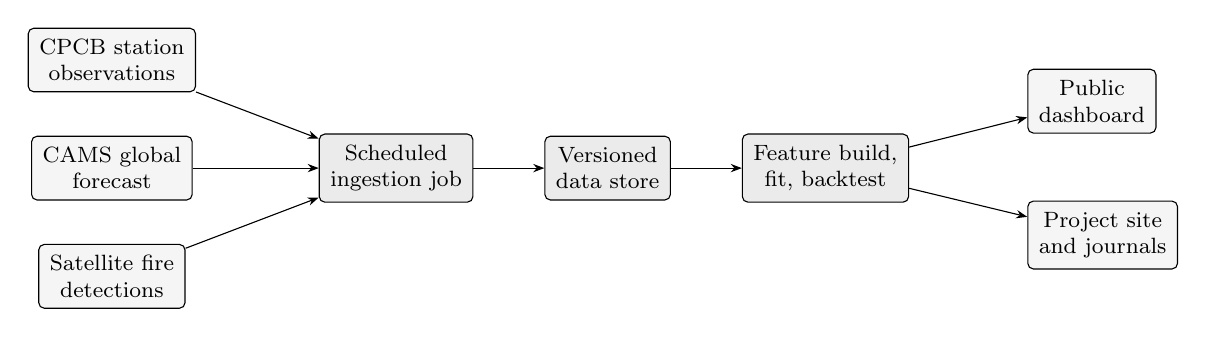
\begin{tikzpicture}[
  node distance=0.55cm and 0.9cm,
  box/.style={draw, rounded corners=2pt, align=center,
    font=\footnotesize, minimum height=0.75cm,
    inner sep=4pt},
  src/.style={box, fill=black!4},
  proc/.style={box, fill=black!8},
  outp/.style={box, fill=black!4},
  ar/.style={-{Stealth[length=4pt]}, thin}
]
\node[src] (cpcb) {CPCB station\\observations};
\node[src, below=of cpcb] (cams) {CAMS global\\forecast};
\node[src, below=of cams] (firms) {Satellite fire\\detections};

\node[proc, right=1.6cm of cams] (ing) {Scheduled\\ingestion job};
\node[proc, right=of ing] (store) {Versioned\\data store};
\node[proc, right=of store] (model) {Feature build,\\fit, backtest};

\node[outp, right=1.5cm of model, yshift=0.85cm] (dash)
  {Public\\dashboard};
\node[outp, right=1.5cm of model, yshift=-0.85cm] (docs)
  {Project site\\and journals};

\draw[ar] (cpcb) -- (ing);
\draw[ar] (cams) -- (ing);
\draw[ar] (firms) -- (ing);
\draw[ar] (ing) -- (store);
\draw[ar] (store) -- (model);
\draw[ar] (model) -- (dash);
\draw[ar] (model) -- (docs);
\end{tikzpicture}%
}
\end{center}

The design is file-based rather than service-based.
Ingested records and computed metrics are stored as
versioned files in the project repository. This has a
useful side effect: every historical state of the
dataset, and every forecast we ever published, remains
auditable afterwards. There is no server to operate and
no database to administer for the duration of the
course.

\subsection{CI/CD as project infrastructure}
Continuous integration and deployment are in place
before the first model is fitted, because the central
artefact of this project is a job that must run by
itself every day.

\begin{itemize}[leftmargin=0.7cm]
  \item A scheduled workflow performs daily ingestion
    without human involvement and records whether it
    succeeded. From week two onward there is a running
    production system, however small.
  \item A workflow on every proposed change runs the
    test suite, covering parser behaviour and schema
    validation of ingested records.
  \item Merging an accepted change rebuilds and
    redeploys both the dashboard and the documentation
    site, so published artefacts cannot drift away from
    the repository.
  \item Credentials live as encrypted repository secrets
    and are injected at run time. They do not appear in
    source at any point.
\end{itemize}

\section{Evaluation Criterion %
\BvrHint{\ldots measurable and attributable}}
Every metric below is computed from timestamped machine
records. None depends on a survey, on self-report, or on
recruiting anyone.

\subsection{Primary metric}
\textbf{Mean absolute error of the next-day mean PM$_{2.5}$
concentration at the Model Town, Patiala station}, in
$\mu$g/m$^3$, over a held-out period, reported as the percentage
reduction against the \emph{persistence} baseline.

Persistence is the primary bar rather than the global forecast,
and the choice is deliberate. Our measurements show the global
forecast is so poorly calibrated here that beating it is not an
achievement: a two-parameter rescale reduces its error by
roughly $84\%$ on the first attempt. Persistence, by contrast,
achieves \PersMAE~$\mu$g/m$^3$, which is $26\%$ of the observed
mean, and is genuinely difficult to improve upon. Setting the
easier reference as the headline would misrepresent the work.

\begin{itemize}[leftmargin=0.7cm]
  \item \textbf{Target, low season:} a reduction of at least
    $10\%$ in MAE relative to persistence, over a held-out
    period drawn from the monsoon and post-monsoon regime.
  \item \textbf{Target, burning season:} a reduction of at least
    $20\%$ relative to persistence during October and November.
    We expect a larger margin here, because day-to-day
    variability rises sharply when transported smoke dominates,
    and persistence degrades fastest in exactly that regime.
    This is the evaluation that matters.
  \item \textbf{Attribution:} model and baselines are scored
    against the same observation series over the same days, so
    differences between them are attributable to the model and
    to nothing else.
\end{itemize}

\subsection{Measured baselines}
The following were computed from public archives over
\NDays{} days, 15 May to 14 August 2026, before any development
began. They fix the ``before'' condition of the project.

\begin{center}
\begin{tabular}{llr}
\toprule
\textbf{Reference} & \textbf{Definition} &
  \textbf{MAE ($\mu$g/m$^3$)} \\
\midrule
Observed mean & mean of observed daily values &
  \ObsMean$^{\dagger}$ \\
Persistence & tomorrow equals today & \PersMAE \\
Climatology & mean of the observed period & \ClimMAE \\
Rescaled CAMS & global forecast, linearly refitted &
  \CamsFitMAE \\
Raw CAMS & global forecast, uncorrected & \CamsMAE \\
\bottomrule
\end{tabular}
\end{center}

\noindent{\footnotesize $^{\dagger}$ a level, not an error;
included so the errors above can be read in proportion.}

\medskip
Three observations follow, and each shaped a design decision.

\begin{itemize}[leftmargin=0.7cm]
  \item Raw CAMS error exceeds the observed mean itself by a
    factor of more than two. The forecast is unusable at this
    station without correction, which establishes that the
    problem is real.
  \item Even optimally rescaled, the global forecast remains
    worse than persistence. Correction of the forecast alone is
    therefore not a viable design, and the model is built around
    local observations instead.
  \item These figures describe the monsoon and post-monsoon
    period, when concentrations are low and stable. They are the
    easy regime. Both baselines will deteriorate substantially
    once burning begins, and we will report the seasonal
    comparison rather than a single annual figure.
\end{itemize}

\subsection{Secondary metrics}
\begin{itemize}[leftmargin=0.7cm]
  \item \textbf{Category recall.} Of the days on which
    observed air quality reached the \emph{Very Poor}
    band or worse, the fraction flagged twenty-four
    hours ahead. The advisory stands or falls on this
    number.
  \item \textbf{False alarm rate.} The fraction of
    issued advisories for days that did not reach the
    flagged band. Reported next to recall so the
    trade-off between the two is visible rather than
    hidden.
  \item \textbf{Pipeline success rate.} The proportion
    of scheduled days on which a forecast was published
    without anyone intervening. This measures the
    engineering, not the model.
  \item \textbf{Data availability.} The proportion of
    expected hourly observations actually received.
    Monitoring stations go offline; we would rather
    report that than quietly drop the rows.
\end{itemize}

\subsection{Validation plan %
\BvrHint{\ldots high-level}}
\begin{itemize}[leftmargin=0.7cm]
  \item Baselines are computed in the first iteration
    from archived data, fixing the ``before'' condition
    ahead of development.
  \item Every iteration is scored on the same held-out
    period, so improvements are comparable across weeks
    rather than only within one.
  \item The final evaluation covers the burning season
    in full. That is the regime the system exists for
    and the hardest test available inside the project
    window.
\end{itemize}

\section{Scalability %
\BvrHint{\ldots with foresight}}

\begin{enumerate}[leftmargin=0.7cm]
  \item \textbf{Scalable in principle.} The design
    generalises along three independent axes without
    structural change.
    \begin{itemize}[leftmargin=0.7cm]
      \item \emph{Spatial.} The monitoring station is a
        configuration value, never a constant in code.
        Additional stations are additional configuration
        entries and additional fits, since the
        correction is per-station by construction.
      \item \emph{Pollutant.} The target variable is a
        parameter. Applying the same method to
        PM$_{10}$ or ozone changes no ingestion or
        evaluation code.
      \item \emph{Horizon.} The upstream forecast
        extends to five days. Extending the corrected
        horizon changes the target column and nothing
        else.
    \end{itemize}
  \item \textbf{Deployable in practice.} The
    substitutions needed to turn this into a maintained
    service are known now, and confined to storage and
    serving.
    \begin{itemize}[leftmargin=0.7cm]
      \item Versioned files become a managed relational
        database with the same schema.
      \item The scheduled repository workflow becomes a
        hosted scheduler.
      \item The static page becomes a small read-only
        API returning the same shape.
      \item Modelling, feature and evaluation code are
        untouched by all three.
    \end{itemize}
\end{enumerate}

\section{Engine availability heuristic}
Everything required is mature, documented and free at
the volume we need. We tested each source before writing
this proposal, and record the outcome here rather than
asserting availability in the abstract.

\begin{itemize}[leftmargin=0.7cm]
  \item \textbf{Ground truth.} The Central Pollution
    Control Board real-time feed, published through the
    national open data platform. Verified to return
    current PM$_{2.5}$ readings for the Model Town,
    Patiala station.
  \item \textbf{Forecast source.} An open API serving the
    CAMS global model. Verified to return a complete
    ninety-two day hourly archive for the Patiala coordinates
    with no missing values. Its accuracy at this station was
    then measured rather than assumed, with the results given
    in Section 6.
  \item \textbf{Fire activity.} NASA's Fire Information
    for Resource Management System, serving satellite
    detections by bounding box. Verified reachable with
    a valid response structure. One caveat surfaced
    during testing and is recorded under risks.
  \item \textbf{Historical observations.} The Central
    Pollution Control Board station archive, used once
    to establish the initial training and baseline
    period.
  \item \textbf{Modelling.} Established open source
    Python libraries for tabular data handling and
    gradient boosted regression.
  \item \textbf{Automation and hosting.} A hosted
    continuous integration runner for scheduled and
    triggered workflows; static hosting for the
    dashboard and documentation.
  \item \textbf{Testing.} A standard Python test
    framework, applied to parsers, schema validation and
    evaluation code.
\end{itemize}

\section{Project scope and deliverables %
\BvrHint{\ldots iteration-friendly}}

\subsection{First iteration}
\begin{itemize}[leftmargin=0.7cm]
  \item Ingestion adapters for the observation feed, the
    forecast source and the fire detection service.
  \item A scheduled workflow appending one validated
    record per day, carrying forecast issue time.
  \item Baselines computed for persistence, climatology
    and the uncorrected forecast over a fixed period.
  \item A first correction model shown to beat
    persistence.
  \item Continuous integration running the test suite on
    every proposed change.
  \item A published dashboard showing corrected and
    uncorrected forecasts for the next day, recent
    observations, current error statistics, and last
    successful run time.
\end{itemize}

\subsection{Later iterations}
\begin{itemize}[leftmargin=0.7cm]
  \item Upwind fire activity and wind direction
    features, introduced ahead of the burning season.
  \item Air quality band classification and the advisory
    rule, with recall and false alarm rate reported
    together.
  \item A rolling-origin backtest covering the full
    season.
  \item Scheduled retraining, with the interval chosen
    from measurement rather than assumed.
  \item Feature importance analysis, used to justify
    keeping or dropping each input.
\end{itemize}

\subsection{Explicitly excluded}
Naming the exclusions is part of defining the scope, and
keeps the deliverable bounded.

\begin{itemize}[leftmargin=0.7cm]
  \item Medical or clinical recommendations of any kind.
    Output is limited to scheduling guidance for outdoor
    activity.
  \item User accounts, authentication, or personal data.
    The service stores nothing about anyone.
  \item Multiple cities within the course window, even
    though the design admits them.
  \item Any modification of the underlying atmospheric
    model, or any claim about atmospheric processes
    beyond the statistical relationship we measure.
\end{itemize}

\section{Risks and mitigations}
\begin{itemize}[leftmargin=0.7cm]
  \item \textbf{Station outage.} Continuous monitoring
    stations drop out, sometimes for weeks. The station
    is a configuration value, so the project can move to
    another Punjab station without code change.
    Availability is reported as a result rather than
    concealed.
  \item \textbf{Distribution shift at season onset.} A
    model fitted on monsoon and post-monsoon air will
    meet a different regime when burning starts. We
    address this with scheduled retraining, and intend
    to report the resulting error trajectory as a
    finding rather than smooth it away.
  \item \textbf{Temporal leakage.} The most serious
    correctness risk, and invisible from performance
    figures alone. Mitigated by recording issue time
    from the first ingestion run and by rolling-origin
    evaluation.
  \item \textbf{Archive retention limits.} Testing
    revealed that the fire detection service serves
    near-real-time and science-quality products under
    different names, with different retention windows,
    and returns an empty result rather than an error
    when a requested date falls outside the window.
    Source selection is therefore driven by the
    availability endpoint rather than hard-coded.
  \item \textbf{Silent interface failure.} Public interfaces
    change without notice, and some fail quietly. During
    development we found that the observation API discards
    unrecognised query parameters rather than rejecting them,
    so a mistyped date filter returned the entire series and
    looked like a successful narrow query. Each source
    therefore sits behind a single adapter that validates the
    \emph{content} of a response, not only its status code,
    and every filtered query is re-checked client side.
  \item \textbf{Ambiguous station identity.} The monitoring
    station is exposed through two sensor identifiers for the
    same pollutant, one of which stopped reporting in 2022 and
    still returns a plausible historical series. The active
    identifier is pinned in configuration with the reason
    recorded, so the choice cannot be silently reversed by
    someone reading the source listing later.
  \item \textbf{Shallow archive of issued forecasts.}
    The accessible archive of issued forecasts is
    bounded, which limits model complexity. We address
    this by preferring low-variance models with few
    parameters, and by beginning automated accumulation
    immediately.
  \item \textbf{Team bandwidth.} Ingestion, modelling
    and delivery each have one responsible member, and
    the pipeline continues collecting data through
    examination weeks without attention.
\end{itemize}

\section{Summary}
We propose a service that corrects a coarse global air
quality forecast at one monitoring station in Patiala,
and publishes the corrected next-day value with a short
advisory.

Against the course criteria: time-to-value is high,
because the evaluation baseline comes from public
archives before development starts and the pipeline
becomes self-sustaining in week two. The evaluation
criterion is measurable and attributable, because
corrected and uncorrected forecasts are scored against
the same observations over the same days. CI/CD is
structural rather than decorative, because the central
artefact is a job that must run unattended every
morning. The engines are mature, free and verified. The
proposition scales along spatial, pollutant and horizon
axes without redesign.

Finally, it is relevant where it is built. The system
addresses a pollution event that occurs in this region
during this semester, and is evaluated against this
region's own monitoring data.

\end{document}
